\documentclass[BCOR20mm,DIV14,twoside,10pt,headinclude,footexclude,bibtotoc,liststotoc]{scrbook}

\usepackage[utf8]{inputenc}
\usepackage[T1]{fontenc}
\usepackage[ngerman]{babel}
\usepackage[final]{pdfpages}
\usepackage{enumitem}

\titlehead{
\centering
\textbf{Universität Ulm}\\
Fakultät für Ingenieurwissenschaften und Informatik\\
Institut für Organisation und Management von Informationssystemen
}

\subject{
    Bachelorarbeit\\
    \footnotesize
    im Studiengang Informationssystemtechnik
}

\makeatletter
\title{Steuerung eines Fussballroboters mit mobilen Endgeräten} \let\thetitle\@title
\author{Patrick Lutz} \let\theauthor\@author
\newcommand\matrikelnr{752774}
\makeatother

\date{
\footnotesize vorgelegt im\\
\normalsize Dezember 2015
}

\publishers{%
\textbf{Gutachter}\\
Prof. Dr. Stefan Wesner\\
}

% Fonts {{{
\usepackage{helvet}             % Helvetica (eig. Nimbus Sans) Klon
\usepackage[sc]{mathpazo}       % Serif Font fuer Texte
\usepackage{microtype}          % Besseres Kerning, weniger Trennungen
% }}}

% Packages {{{
\usepackage{graphicx}
\usepackage{amsmath, amsthm, amssymb}
\usepackage{listings}
\usepackage{multicol}
\usepackage{booktabs}
\usepackage{url}
\usepackage{ccicons}
\usepackage{gensymb}

\usepackage{natbib}
\setcitestyle{square,numbers,comma,sort}
% }}}

% Bildunterschriften {{{
\usepackage{caption}   % Sans-Serif Font fuer Bildunterschriften
\captionsetup{labelfont={sf,bf},font=sf}
\usepackage[sf,bf,SF]{subfigure}
% }}}

% Bilder {{{
\usepackage{tikz}
% }}}

% Satzspiegel {{{
\renewcommand{\baselinestretch}{1.10}
\setlength{\parindent}{0pt}
\setlength{\parskip}{\baselineskip}
\widowpenalty10000
\clubpenalty10000
% }}}

% Ueberschriftstiefe im TOC
\setcounter{tocdepth}{2}

% Literaturverzeichnis
\bibliographystyle{dinat}

% Kopf- und Fusszeilen {{{
\usepackage{scrpage2}
\pagestyle{scrheadings}
\clearscrheadfoot
\setkomafont{pagehead}{\sffamily}
\automark[section]{chapter}
\ohead{\headmark}
\ofoot{\pagemark}
\setheadsepline{.4pt}
% }}}

% PDF Eigenschaften {{{
\makeatletter
 \usepackage[pdftex,
 	unicode=true,
 	colorlinks=true,
 	linkcolor=black,
 	citecolor=black,
 	urlcolor=black,
 	pdfauthor={\@author}
 ]{hyperref}
\makeatother
% }}}

% Nuetzliche Befehle {{{
\newcommand{\etal}{\emph{et\,al.}}
\newtheorem{defn}{Definition}[chapter]
\newtheorem{thm}{Satz}[section]
% }}}

\hyphenation{%
Fahr-zeug-zu-In-fra-struk-tur-Kom-mu-ni-ka-ti-on
}


\begin{document}

\frontmatter %%%%%%%%%%%%%%%%%%%%%%%%%%%%%%%%%%%%%%%%%%%%%%%%%%%%%%%%%%%%%%%%%%
%\maketitle
\thispagestyle{empty}

\newlength{\backup}
\setlength{\backup}{\headheight}
%\setlength{\headheight}{42mm}


\includegraphics[height=1.8cm]{images/logo_100_sw_bildmarke}
\hfill

\includegraphics[height=1.8cm]{images/logo_100_sw_wortmarke}\\[1em]

{\footnotesize
\hspace*{10.85cm}{\bfseries Fakultät für\\
\hspace*{10.85cm}Ingenieurwissenschaften\\
\hspace*{10.85cm}und Informatik}\\
\hspace*{10.85cm}Institut für Organisation und\\
\hspace*{10.85cm}Management von Informations-
\hspace*{10.85cm}systemen\\[1em]
\hspace*{10.85cm}Dezember 2015\\[6em]
}
{\bfseries \huge Steuerung eines Fussballroboters mit \\ mobilen Endgeräten\\
}\\[0.5em]
{\large Bachelorarbeit an der Universität Ulm}\\[1em]
OMI-2015-12-31\\[4em]

%{\large \bfseries ENTWURF: \today}
%\\[2em]

{\large \bfseries Vorgelegt von:}\\                     
\theauthor \\[2em]
{\large \bfseries Gutachter:}\\                     
Prof. Dr. Stefan Wesner\\
\\[2em]
{\large \bfseries Betreuer:}\\ 
Dipl.-Inf. Lutz Schubert\\


\newpage
\setlength{\headheight}{\backup}


\thispagestyle{empty}

{% impressum
  \newpage
  \small
  \flushleft
  \mbox{}\\\vspace{180mm}

  Fassung \today \\
  {\normalsize \copyright~2014 \theauthor}\\
  %
This work is licensed under the Creative Commons Attribution-NonCommercial-ShareAlike 2.0 License. To view a copy of this license, visit http://creativecommons.org/licenses/by-nc-sa/2.0/de/ or send a letter to Creative Commons, 543 Howard Street, 5th Floor, San Francisco, California, 94105, USA. \\
  %
  Satz: PDF-\LaTeXe
}


\pagestyle{scrheadings}

\clearscrheadfoot
\ohead{\headmark}
\cfoot[\pagemark]{\pagemark}

\chapter*{Abstract}
...

\tableofcontents

\mainmatter %%%%%%%%%%%%%%%%%%%%%%%%%%%%%%%%%%%%%%%%%%%%%%%%%%%%%%%%%%%%%%%%%%%

\chapter{Einleitung}
\label{ch:einleitung}

Die Geschichte der Roboter reicht bis in die Antike zurück. Schon dort gab es erste Versuche mit Automaten, die zum Beispiel Musik spielen sollten oder automatisch Theater spielen konnten. Mit dem Verlust der antiken Kulturen gingen jedoch auch die Kenntnisse über die Automation verloren. Erst im 13. Jahrhundert wurde ein Buch eines arabischen Ingenieurs bis in die westliche Welt bekannt, was Gerüchten zufolge auch Leonardo da Vinci für die Automation inspiriert haben soll. 
Roboter wie wir sie kennen gibt es erst seit Mitte des 20. Jahrhunderts. Der technische Wendepunkt, der mit der Erfindung des Transistors kam, machte es erst möglich, elektrische Schaltungen in einer Größe zu fertigen, die für Roboter notwendig ist. Seit diesem Zeitpunkt liegt ein wertvoller und nicht mehr wegzudenkender Industriezweig auf dem Gebiet der Robotik. Mit dem Einstieg der Robotik in die Industrie wurde die Produktion um ein vielfaches schneller und präziser, als sie von Menschenhand je vorgenommen werden könnte. Auch in Bereichen oder Umgebungen, die für Menschen lebensgefährlich oder ohnehin lebensunmöglich sind, spielen Roboter eine bedeutende Rolle. Ein Beispiel hierfür ist der Mars-Rover. Der Mars-Rover ist ferngesteuertes Fahrzeug, welcher für die Marsforschung verwendet wird und größten Teils von der Erde aus gesteuert wird. Wie die meisten ferngesteuerten Fahrzeuge ist er mit einer Vielzahl von Sensoren und Werkzeugen ausgestattet. 

Seit Ende der 90-er Jahre gibt es einen weltweiten Wettbewerb namens RoboCup. Bei RoboCup geht es darum, ein Fussballspiel von Robotern austragen zu lassen. Diese Bachelorarbeit beschäftigt sich ebenfalls mit dem Thema der Steuerung von mobilen Robotern mit dem Ziel, ein Roboter-Fussballspiel zu ermöglichen. Im Gegensatz zum RoboCup, bei dem die Roboter entweder autonom, oder von einem zentralen Computer gesteuert werden, der mittels einer Kamera über dem Spielfeld die Bewegungen und Situationen erfasst, wird in dieser Bachelorarbeit die Steuerung der Roboter vom Menschen übernommen. Auf einer Tischplatte in der Universität sollen zwei Roboter platziert werden. An den beiden Enden der Tischplatte werden Tore montiert, ähnlich wie man es beim Tischfussball kennt. Mithilfe von mobilen Endgeräten sollen nun die Roboter angesteuert werden können und ein Zwei-Spieler Fussballspiel ermöglicht werden. Die Roboter verfügen über einen Schussapparat, der es möglich macht den Ball zu beschleunigen. Sobald der Ball in ein Tor befördert wurde, wird ein Tor automatisch erkannt und auf den mobilen Endgeräten, welche die Steuercontroller bilden, angezeigt. Diese Steuercontroller können entweder ein Android-Gerät oder jedes beliebige andere Gerät sein, das über eine Tastatur und einen Webbrowser verfügt. Über diese Steuercontroller ist es möglich die Roboter zu navigieren und einen Schuss zu tätigen. Hierfür werden verschiedene Steuerarten bereitgestellt. 
Die Roboter bewegen sich vollkommen kabellos, was die Verwendung eines Akkus notwendig macht. Sobald der Akku einen Mindestprozentsatz unterschreitet, wird automatisch die Ladestation angefahren, damit sich der Akku des Roboters selbstständig, also ohne menschliches Eingreifen, lädt.
Die Fertigung und Implementierung der Roboter ist Teil einer anderen Bachelorarbeit, auf die hier nur Oberflächlich eingegangen wird.               

% hier kommt noch ein kurzer überblick über die arbeit, welche kapitel folgen und was in welchen kapiteln ungefähr beschrieben wird




\section{Anforderungen}
Das Ziel der Bachelorarbeit ist es, ein Fussballspiel für zwei Spieler zu realisieren. Hierfür werden zwei Roboter auf einem begrenzten Spielfeld positioniert. Jeweils am Rand des Spielfelds wird ein Tor montiert, in das der Ball befördert werden soll. Mittels mobilen Endgeräten und herkömmlichen PCs soll es möglich sein, die Steuerung über einen der Roboter zu übernehmen. Sobald beide Roboter mit einem Steuergerät verbunden sind, soll ein Spiel gestartet werden und die Torerkennung funktionieren. Das bedeutet, sobald ein Spieler ein Tor erzielt hat, erkennt das System dieses und erhöht den Spielstand dementsprechend. Mittels einer Kamera, die auf den Robotern montiert ist, soll eine Videoübertragung aus Sicht der Roboter stattfinden. Dadurch soll es auch möglich sein, die Roboter zu steuern, ohne sich in Sichtkontakt mit den Robotern zu befinden. Da die Roboter über einen Akku verfügen, soll die Kommunikation kabellos erfolgen, damit ein freies Fahren der Roboter sichergestellt ist. Weil der Akku eine begrenzte Kapazität hat, soll der Roboter bei niedrigem Akkustand selbstständig die Ladevorrichtung anfahren und während der Ladezeit keine Steuerbefehle annehmen. Aufgrund der Interaktion mit menschlichen Benutzern, ist es wichtig, dass der Roboter eine möglichst rechtzeitige Steuerung darstellt, um Verzögerungen und die dadurch entstehende Unkontrollierbarkeit zu vermeiden.


\section{Schnittstelle zum Roboter}
\label{sec:schnittstelle}
                                                                                                                                                                                                                                                                                                                                                                                                                                                                                                                                                                                                                                                                                                                                                                                                                                                                                                                                                                                                                                                                                                                                                                                                                                                                                                                                                                                                                                                                                                                                                                                                                                                                                                                                                                                                                                                                                                                                                                                                                                                                                                                                                                                                                                                                                                                                                                                                                                                                                                                                                                                                                                                                                                                                                                                                                                                                                                                                                                                                                                                                                                                                                                                                                                                                                                                                                                                                                                                                                                                                                                                                                                                                                                                                                                                                                                                          
                                                                                                                                                                                                                                                                                                                                                                                                                                                                                                                                                                                                                                                                                                                                                                                                                                                                                                                                                                                                                                                                                                                                                                                                                                                                                                                                                                                                                                                                                                                                                                                                                                                                                                                                                                                                                                                                                                                                                                                                                                                                                                                                                                                                                                                                                                                                                                                                                                                                                                                                                                                                                                                                                                                                                                                                                                                                                                                                                                                                                                                                                                                                                                                                                                                                                                                                                                                                                                                                                                                                                                                                                                                                                                                                                                                                                                                          
                                                                                                                                                                                                                                                                                                                                                                                                                                                                                                                                                                                                                                                                                                                                                                                                                                                                                                                                                                                                                                                                                                                                                                                                                                                                                                                                                                                                                                                                                                                                                                                                                                                                                                                                                                                                                                                                                                                                                                                                                                                                                                                                                                                                                                                                                                                                                                                                                                                                                                                                                                                                                                                                                                                                                                                                                                                                                                                                                                                                                                                                                                                                                                                                                                                                                                                                                                                                                                                                                                                                                                                                                                                                                                                                                                                                                                                                                                                                                                                                                                                                                                                                                                                                                                                                                                                                                                                                                                                                                                                                                                                                                                                                                                                                                                                                                                                                                                
% ...

\chapter{Grundlagen}
\label{ch:Grundlagen}


UDP

Beim User Datagram Protocol handelt es sich um ein verbindungsloses und in jeglicher Hinsicht ungeschütztes Protokoll, das auf der Transportebene (Schicht 4 im OSI-Schichtenmodell) arbeitet. Es bestehen keinerlei Mechanismen, die das korrekte Übertragen von Paketen gewährleisten. Hierzu zählen:

\begin{description}
	\item[Sicherheit] Die Sicherheit, dass Pakete überhaupt ankommen
	\item[Reihenfolge] Die Reihenfolge, in der Pakete ankommen
	\item[FlowControl] Ein Überlaufschutz des Empfängerspeichers (FlowControl)
	\item[CongestionControl] Stauvermeidung in der Übertragungskette (CongestionControl)
	\item[Angriffe] Schutz gegen Paketmanipulation von dritten
\end{description}

\begin{figure}
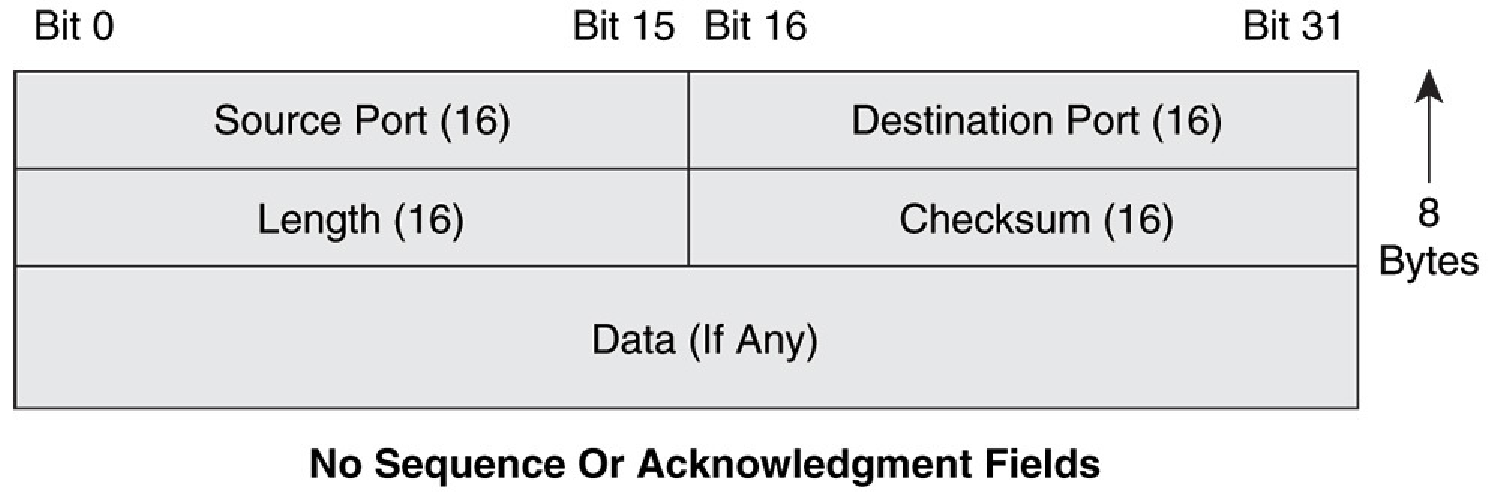
\includegraphics[width=\textwidth]{images/UDP_header.pdf}
\caption{UDP Header}
\label{fig:udp_header}
\end{figure}

Ein UDP Header besteht aus 8 Byte. Mit diesen 8 Byte werden lediglich Source-Port, Destination-Port, Länge und die Checksumme übertragen. Dieser vergleichsweise kleine Header (vgl. TCP mit etwa 20 Byte), führt zu einem geringen Overhead während der Übertragung, auch bei kleinen Paketen. Nachdem ein Paket gesendet wurde erfolgt keine Bestätigung des Pakets vom Empfänger. Durch diesen Uni-Direktionalen Sendevorgang entsteht wenig Traffic im Netzwerk. Falls gewisse Sicherheitsmechanismen gewünscht sind, müssen diese in höheren Schichten implementiert werden. \\
Aufgrund dieser Eigenschaften wird UDP in Bereichen eingesetzt, in denen es auf hohe Übertragungsgeschwindigkeit ankommt und eventuelle Paketverluste zu verkraften sind, bzw. von höheren Schichten aufgelöst werden.




\newpage


TCP

Beim Transmission Control Protocol handelt es sich um ein verbindungsorientiertes paketvermittelndes Protokoll. Mithilfe verschiedener Mechanismen wird sichergestellt, dass Pakete in der richtigen Reihenfolge ankommen, es zu keinen Staus kommt und dass Netzwerkknoten nicht überlaufen. Dadurch, dass das Protokoll verbindungsorientiert arbeitet, können beide Teilnehmer der Verbindung Daten ohne Anfragen senden. 

\begin{figure}
	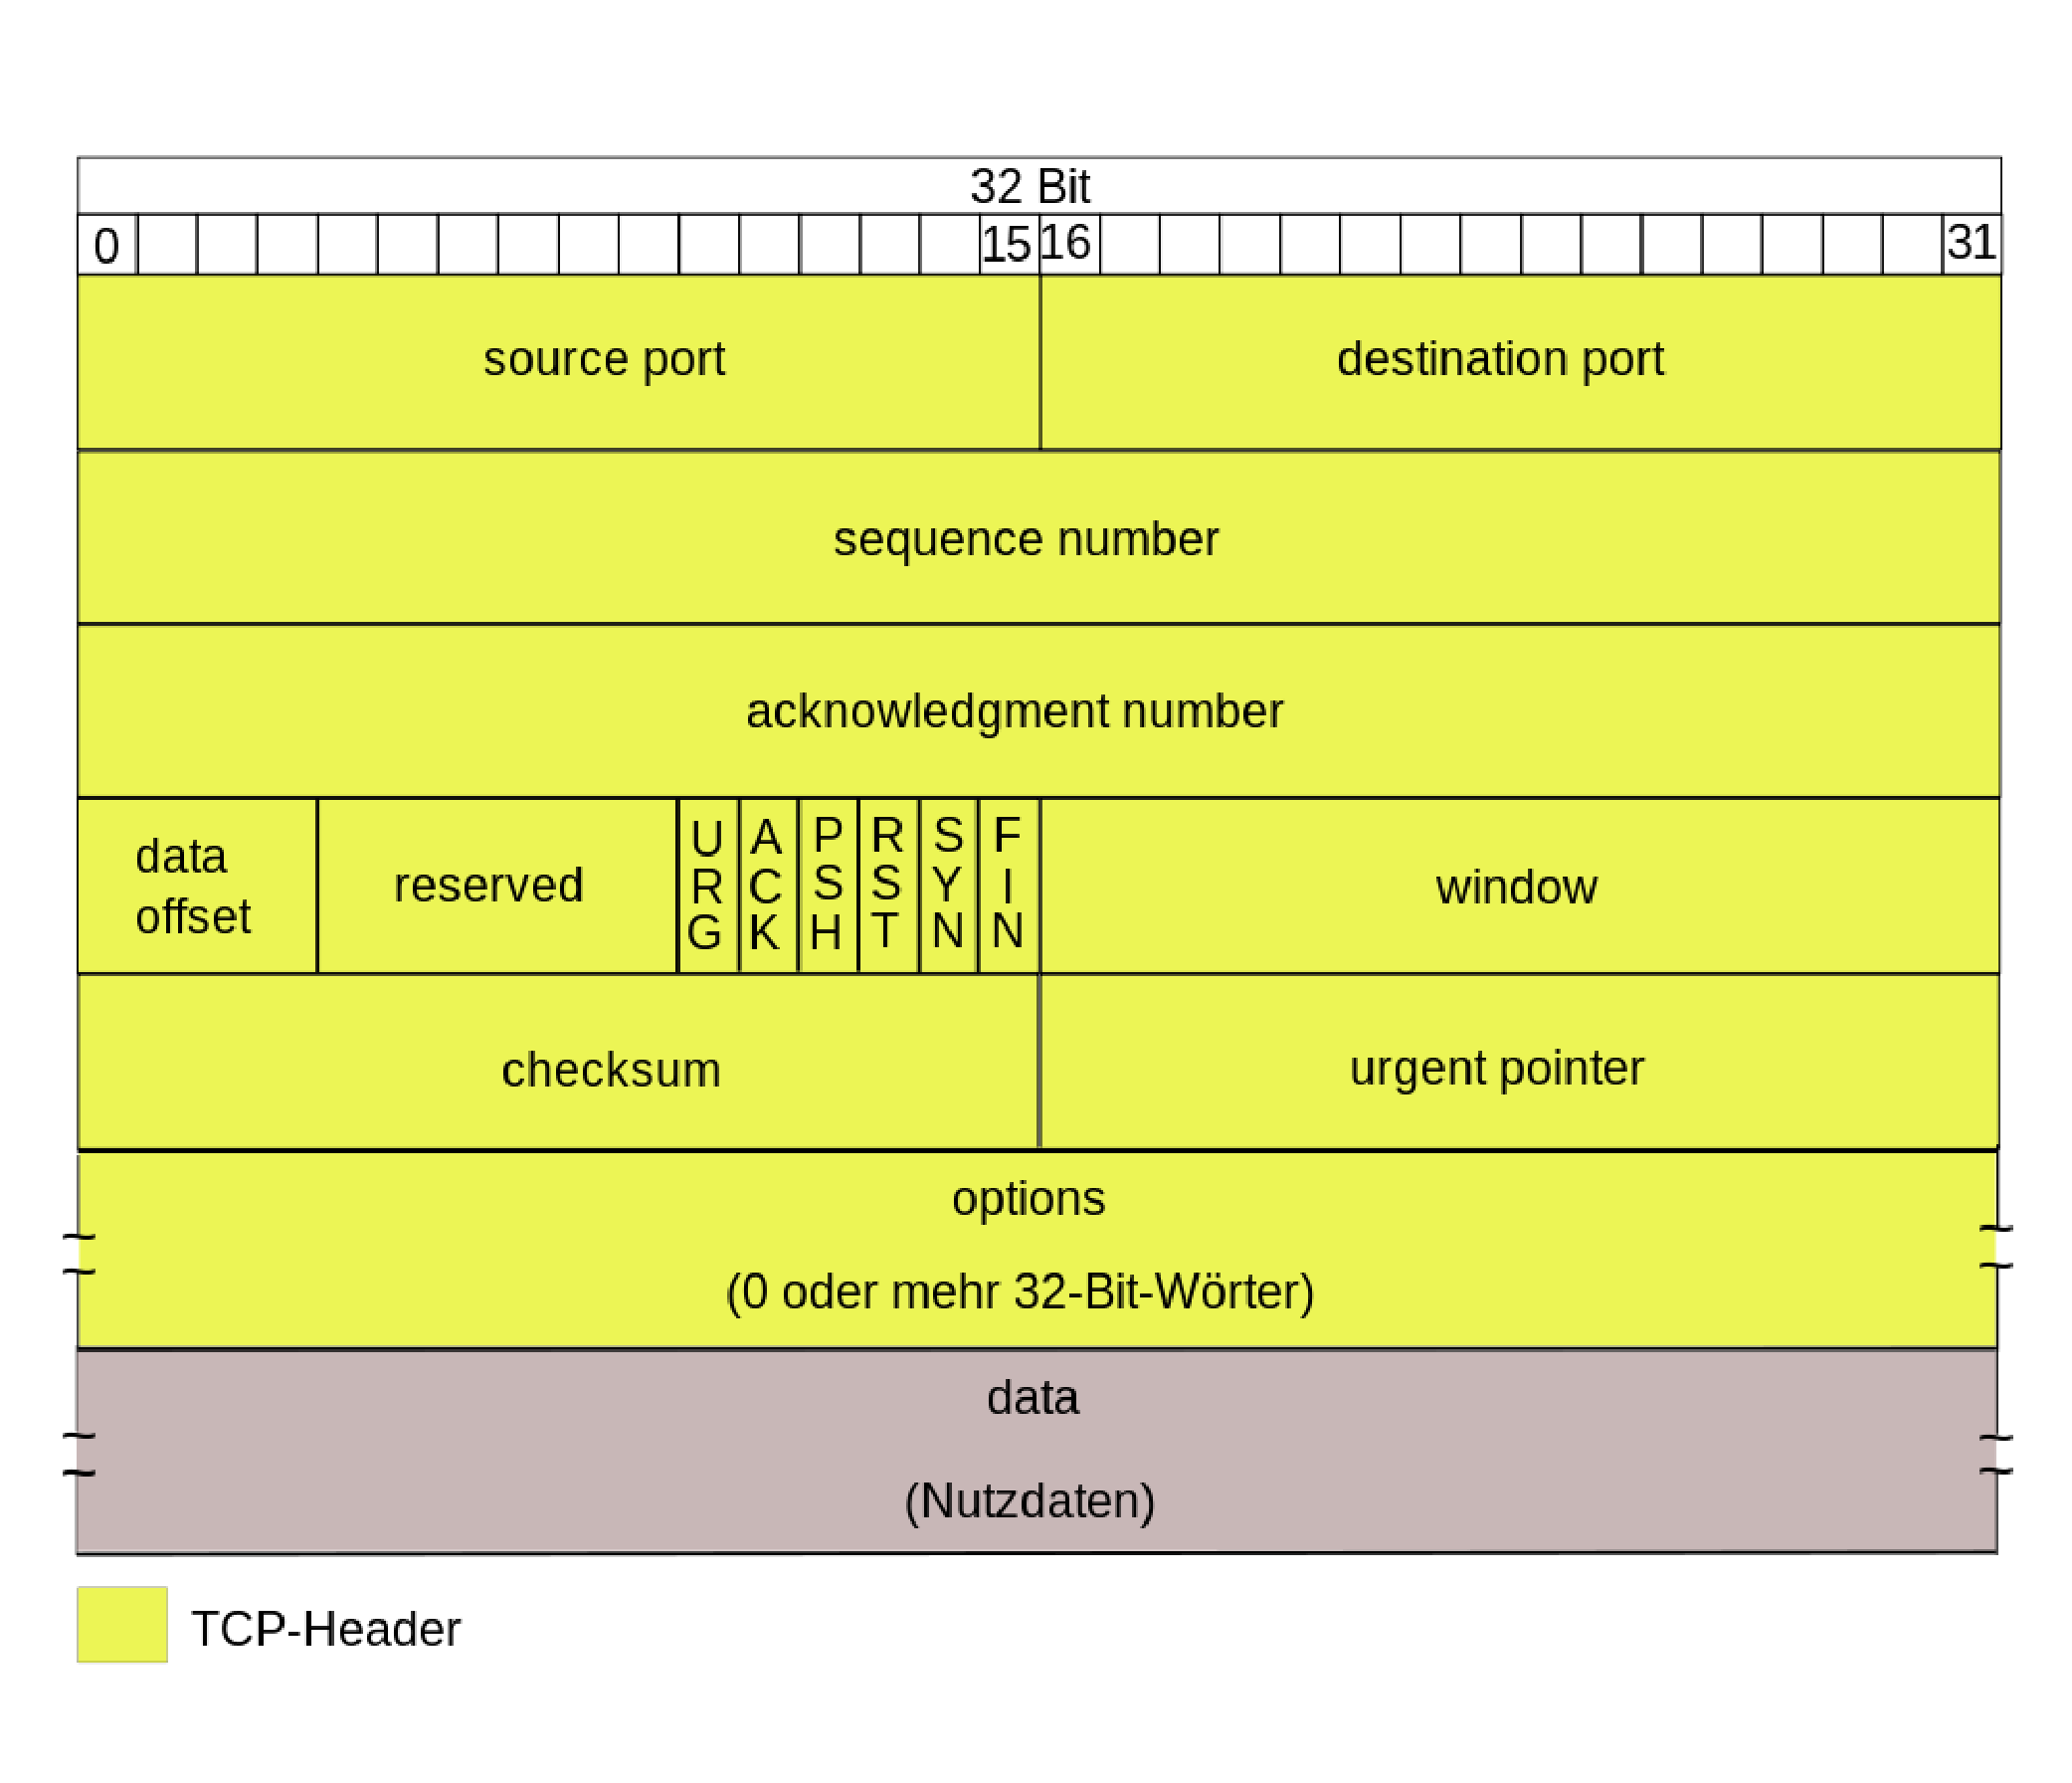
\includegraphics[width=\textwidth]{images/TCP_header.pdf}
	\caption{TCP Header}
	\label{fig:tcp_header}
\end{figure}

Durch den größeren Header und dem größeren Traffic, der das Protokoll verursacht, wird TCP für Anwendungen verwendet, bei denen ein Paketverlust ausgeschlossen werden soll, dafür aber eine etwas höhere Latenz in Kauf genommen werden kann. 
Die Verbindung wird über einen 3-Wege-Handshake hergestellt. Hierbei sendet ein Teilnehmer eine Anfrage (syn), diese wird bestätigt (syn ack) woraufhin die Bestätigung erneut bestätigt wird. In diesem dritten Schritt werden meist bereits die ersten Nutzdaten mitgesendet.
\begin{figure}
	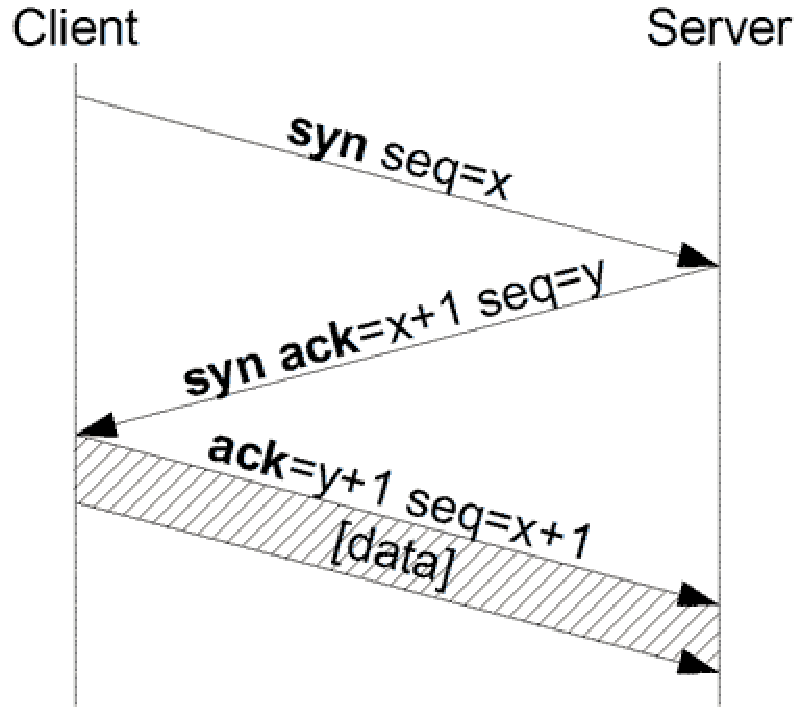
\includegraphics[width=\textwidth]{images/TCP_3wayhandshake.pdf}
	\caption{TCP 3-Wege-Handshake}
	\label{fig:tcp_3wayhandshake}
\end{figure}

Mithilfe von geordneten Sequenznummern und Acknowledgments werden alle empfangene Pakete bestätigt. Durch das Fehlen einer Sequenznummer erkennt der Empfänger den Verlust eines Pakets und teilt daraufhin dem Sender mit, dass es nicht angekommen ist. Für den Fall eines Verlusts des Acknowledgments, hat der Sender einen Timer, welcher nach einiger Zeit eine Retransmission des Pakets veranlasst, sofern kein Acknowledgment ankommen sollte.




HTTP

Das Hypertext Transfer Protocol ist ein zustandsloses Datenübertragungsprotokoll, das auf der Anwendungsschicht arbeitet. Am meisten wird das Protokoll für den Aufbau von Internetseiten verwendet, also von einem Webbrowser, jedoch ist das Aufgabenfeld nicht darauf beschränkt.

HTTP arbeitet mittels zwei Befehlsarten, dem Request und dem Response. Möchte ein Browser eine Datei von einem Server laden, so sendet er einen Request mit dem Namen der Datei. \\
Die möglichen Befehle sind: 
\begin{description}
	\item[GET] fordert eine Ressource auf dem Server an
	\item[POST] sendet Daten zur weiteren Verarbeitung zum Server
	\item[HEAD] fordert lediglich den HEADER eines Responses an, der auf einen GET-Request folgend würde
	\item[PUT] lädt eine Ressource auf den Server
	\item[DELETE] löscht eine Ressource auf dem Server (Wird kaum verwendet)
	\item[TRACE] sendet die Anfrage, so wie sie empfangen wurde zurück
	\item[OPTIONS] liefert eine Liste mit den vom Server unterstützten Optionen
	\item[CONNECT] wird für SSL-Tunneling verwendet
\end{description} Nachdem der Request beim Server eingegangen ist und verarbeitet wurde, sendet er einen Response. In diesem Response sind Informationen über Server und Datei enthalten, sowie die Nutzdaten, also die angefragte Datei. In Abbildung \ref{fig:http_request_response} ist eine solche Kommunikation dargestellt.
-- 
\begin{figure}
	\includegraphics[width=\textwidth]{images/http_request_response.pdf}
	\caption{HTTP Kommunikation}
	\label{fig:http_request_response}
\end{figure}



WebSockets

Das WebSocket-Protokoll ist ein Netzwerkprotokoll, das auf TCP und HTTP basiert. In diesem Protokoll ist es möglich, eine bidirektionale Verbindung zwischen einer Webanwendung und einem WebSocket-Server herzustellen. Im Gegensatz zu reinem HTTP ist es hierbei möglich, dass der Server ohne einen vorhergehenden Request des Clients, Daten an den Client sendet. Lediglich den Verbindungsaufbau muss der Client initiieren. Dies wird realisiert, indem die TCP-Verbindung nach dem Verbindungsaufbau nicht sofort geschlossen wird. 
Eine WebSocket URL wird über die beiden Schemata wss und ws definiert, was für verschlüsselte und unverschlüsselte Verbindungen steht.

Der Verbindungsaufbau funktioniert über einen Handshake, der wie in HTTP üblich über einen Request und anschließenden Response erreicht wird. Aufgrund der Tatsache, dass die HTTP-Header nur beim Verbindungsaufbau gesendet werden und dadurch der Traffic durch den HTTP-Header gering ist, wird das Protokoll hauptsächlich von Anwendungen verwendet, die regelmäßige Kommunikation zwischen Client und Server verlangen, wie zum Beispiel Online-Spiele.



Jetty Webserver

Jetty ist eine Java-Implementierung eines Webservers. Durch seine geringe Größe ist es leicht, ihn in andere Software zu integrieren. Außerdem unterstützt Jetty die Möglichkeit WebSockets aufzubauen.
% ...

\chapter{Software Architektur}
\label{sec:software-architektur}

Die Software-Architektur des Projektes definiert die Möglichkeiten bei der Implementierung, die man zum Erfüllen der Anforderungen zur Verfügung hat. Deshalb war es wichtig, sich ausreichend Gedanken zu machen, um später im Projekt dann nicht feststellen zu müssen, dass die gewählte Architektur für die Anforderungen ungeeignet ist. Die Hauptanforderung an die Architektur ist selbstverständlich die Bereitstellung eines Kommunikationskanals zwischen Controllern und Robotern. Es muss möglich sein Richtungs- und Geschwindigkeitsänderungen seitens der Anwender rechtzeitig an die Roboter mitzuteilen. Der Status des Roboters soll jederzeit ausgewertet und entsprechend darauf reagiert werden können. Hierzu gehören das automatische Anfahren der Ladestation bei geringem Akkustand und die Übertragung der Bilddaten. Außerdem sollen Zustandsänderungen des Spiels, die nicht vom Roboter oder Controller direkt ausgehen erkannt und korrekt verarbeitet werden. 

Ausgehend von diesen Bedingungen, die die Architektur erfüllen muss, kamen folgende Architekturen in Frage:

Eine \textbf{Client-Server-Architektur} bei der ein Server zentral die Kommunikation verwaltet. Hierbei findet keine Kommunikation zwischen den Steuergeräten und den Robotern direkt statt. Die Torerkennung kommuniziert direkt mit dem Server, ohne dass Roboter und Controller zwangsweise etwas davon mitbekommen. Sowohl die Roboter, als auch die Controller nehmen die Rolle eines Clients ein. Dadurch ist es Möglich, dass eine Steuerung des Servers stattfinden kann, ohne dass ein Controller verbunden ist. Zusätzlich ist es in dieser Architektur möglich beliebig viele Clients anzubinden. Durch die Trennung von Client und Logik können die Controller beliebig erweitert und ausgetauscht werden, ohne die eigentliche Spiellogik zu ändern.

\begin{figure}[!h]
	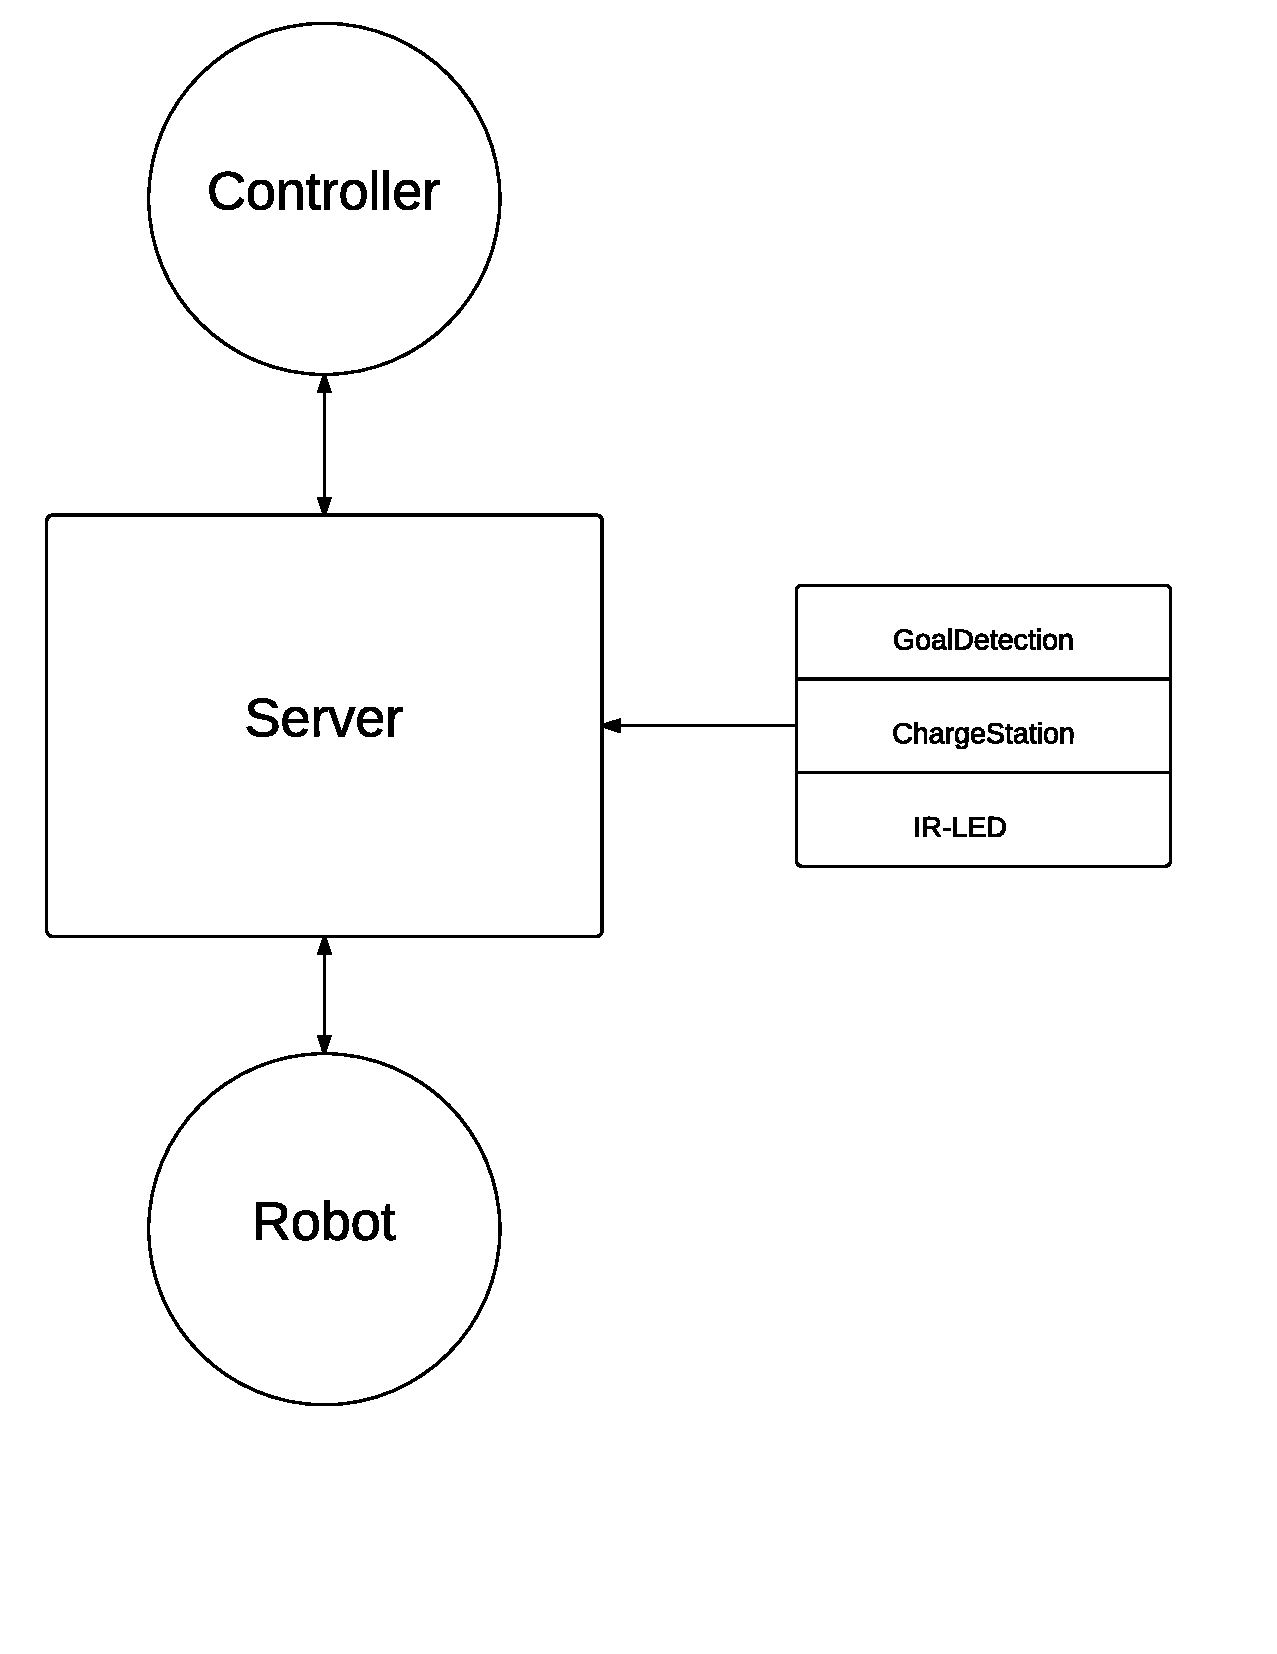
\includegraphics[scale=0.25]{images/client-server_architektur.pdf}
	\caption{Client-Server Architektur}
	\label{fig:client-server_architektur}
\end{figure}


Eine Architektur, die Roboter und Controller \textbf{paarweise} verbindet. Bei dieser Architektur wird jedem Roboter ein Controller zugewiesen, der genau diesen steuert. Die peripheren Geräte senden direkt an die Controller. Auch die gesamte Spiellogik ist in den Controller gekapselt. Ein Vorteil dieser Architektur ist die geringe Latenz bei der Befehlsübermittlung. Im Vergleich zur Client-Server-Architektur gibt es hier keinen dritten Knoten, über den die Übertragung abgehalten wird, wodurch sich die benötigte Zeit halbiert. Dies stellt für die Rechtzeitigkeit der Steuerung einen erheblichen Vorteil dar.

\begin{figure}[h!]
	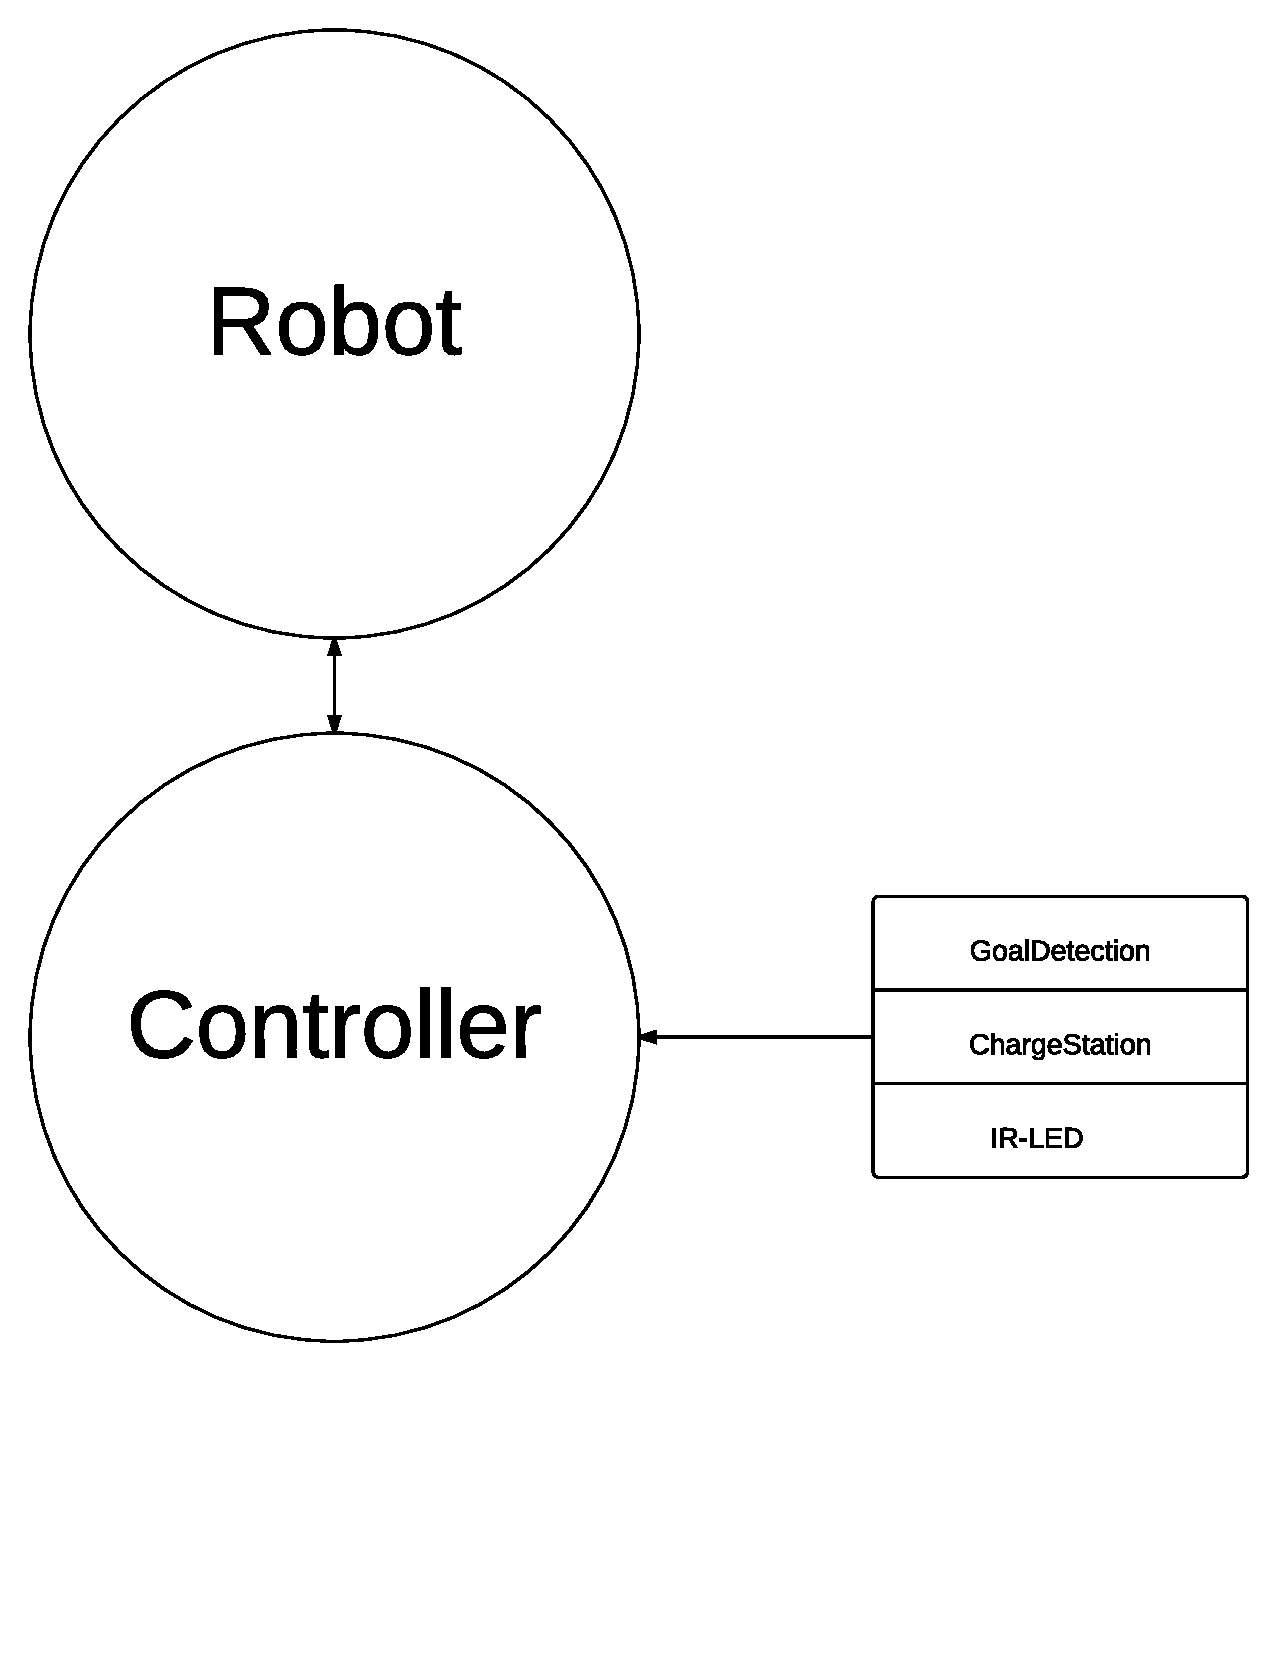
\includegraphics[scale=0.25]{images/paarweise_architektur.pdf}
	\caption{Paarweise Architektur}
	\label{fig:paarweise_architektur}
\end{figure}


Nach Abwägung der Vor- und Nachteile beider Architekturen schien es vernünftiger sich für die Client-Server-Architektur zu entscheiden. Einer der Hauptgründe hierfür ist die hervorragende Erweiterbarkeit in Bezug auf die Controller. Da keine Logik in den Controllern ist, muss sie auch nicht für jeden Controller separat entwickelt werden, beziehungsweise nicht einmal vorhanden sein. Gerade für das Auffinden der Ladestation wäre es nicht sinnvoll, solange mit dem Laden zu warten, bis ein Controller verbunden ist, nur um dann festzustellen dass der Akku leer ist und der Roboter erst geladen werden muss, bevor gespielt werden kann. Auch in Anbetracht der Informationskapselung, die bei der paarweisen Architektur entstehen würde, ist es sinnvoller die Client-Server-Architektur zu bevorzugen. Nur wenn alle Informationen über das Spiel, also über jeden Roboter und jeden Controller zentral verwaltet werden, ist es möglich die Informationen korrekt zu verarbeiten und entsprechend darauf zu reagieren. So wird zum Beispiel ein neues Spiel gestartet, sobald beide Roboter mit einem Controller verbunden sind. Bei der paarweisen Architektur wäre dies nicht möglich, da die beiden Controller-Roboter-Einheiten vom jeweils anderen keine Informationen über deren Status erhalten. In Anbetracht der Rechtzeitigen Steuerung bietet die gewählte Architektur einen Nachteil gegenüber der paarweisen. Jedoch wird sich später bei der Implementierung herausstellen, dass die Übertragungsgewschwindigkeit auch bei der Client-Server Architektur hoch genug ist, um eine für den Benutzer verzögerungslos erscheinende Steuerung zu gewährleisten.
% ...

\chapter{Kommunikation}
\label{sec:kommunikation}

\subsection*{Übertragungstechnologie}
Da die Roboter, sowie auch die Controller über Funk mit dem Server kommunizieren sollten, gab es an dieser Stelle einige Entscheidungen. \\
Generell musste hierbei zwischen der Roboter-Server und der Controller-Server Kommunikation unterschieden werden. Für beide Wege gab es verschiedene Anforderungen. 
Da der Server in Nähe der Roboter aufgestellt werden soll spielt hierbei die Übertragungsdistanz keine sehr große Rolle, weshalb Bluetooth denkbar wäre, auch WLAN wäre eine gute Lösung, da in den meisten Gebäuden ein drahtloses Netzwerk vorhanden ist. Selbst optische Übertragungsverfahren wären denkbar (und werden sogar verwendet, siehe Kapitel %TODO ladestation
).

Die Hauptanforderungen an die Roboter-Server Übertragung sind Übertragungsgeschwindigkeit und Ausfallsicherheit. Eine energiesparende Lösung ist aufgrund der begrenzten Akkukapazität der Roboter wünschenswert. \\
Da die Roboter ständig in Bewegung sind und Richtungsänderungen schnell und zuverlässig verarbeitet werden sollen, wurde die optische Übertragung ausgeschlossen. Bei einem solchen Verfahren müsste ein ständiger Sichtkontakt zwischen Sender und Empfänger bestehen, was eine robuste Übertragung beim Fahren um Hindernisse nahezu ausschließt. \\
 Bluetooth würde die Anforderung der Ausfallsicherheit erfüllen, da die Roboter auf einem begrenzten Gebiet zum Einsatz kommen und die Distanz deshalb ausreichend gering wäre. Auch in Punkto Energieeffizienz wäre mit Bluetooth Low Energy eine gute Lösung gefunden, da es im Vergleich zu WLAN beim Senden nur in etwa ein sechstel des Stroms verbraucht %TODO( Quelle MUC )
. \\
WLAN bringt eine hohe Ausfallsicherheit, da die Verbindung in Gebäuden als nahezu Konstant anzunehmen ist. Da der Server im gleichen Netzwerk hängt wie der Roboter, ist es bei dieser Übertragung irrelevant wie weit die beiden Geräte tatsächlich voneinander entfernt sind, solange sie sich eben im selben Netzwerk befinden, was gegenüber Bluetooth mehr Spielraum für die Größe des Spielfeldes übrig lässt. Was die Übertragungsgeschwindigkeit angeht, ist WLAN um ein vielfaches schneller (stark von Version abhängig). \\

Aufgrund der besseren Flexibilität und der höheren Übertragungsrate fiel an dieser Stelle die Entscheidung auf \textbf{WLAN}. Der Vorteil von Bluetooth bestünde hier lediglich in der besseren Energieeffizienz, jedoch ist die Akkubelastung, die durch die Kommunikation eintritt im Vergleich zu der der Motoren wesentlich geringer. Dadurch fällt die vergleichsweise hohe Belastung von ca. 300mA bei WLAN im Gegensatz zu ca 50mA bei Bluetooth (beim Sendevorgang) nicht so sehr ins Gewicht, wie der Stromverbrauch, der durch die Motoren und den Schussapparat verursacht wird. %TODO nachfragen wieviel die überhaupt ziehen, nicht dass die kaum was brauchen und ich den akku mit befehlen leer zieh..


Für die Kommunikation zwischen Controller und Server gelten prinzipiell die gleichen Anforderungen, jedoch andere Rahmenbedingungen. Zusätzlich soll es möglich sein den Server mit seinem Controller auch außerhalb der Universität zu erreichen. Da die mobilen Endgeräte in den meisten Fällen ebenfalls über einen Akku mit Strom versorgt werden, spielt hier auch der Aspekt der Energieeffizienz eine Rolle. Weil die Controller den Server aber auch von weiter entfernten Orten erreichen sollen, die auch außerhalb der Universität liegen können, ist hier lediglich eine Kombination verschiedener Übertragungstechnologien möglich. Deshalb fiel die Entscheidung hierbei ebenfalls auf die Netzwerkvariante, da hiermit das Übertragungsmedium keine entscheidende Rolle spielt. So ist es zum Beispiel möglich sich von zu Hause mittels VPN Zugang zum Universitäts-Netzwerk zu verschaffen. Diese Entscheidung erlaubt es auf Netzwerkebene zu agieren, ohne sich über die Data-Link Layer Gedanken machen zu müssen.




\subsection*{Übertragungsprotokoll}
Nach der Entscheidung über die Übertragungstechnologie blieben für die Wahl des Übertragungsprotokolls grundlegend nur wenige Protokolle zur Auswahl. Diese sind UDP und TCP. Alle anderen denkbaren Protokolle basieren letztendlich auf einem der beiden und stellen nur Erweiterungen dar.

Bei der Roboter-Server Kommunikation gibt es hierbei einige Dinge zu berücksichtigen. In der Richtung Server-zu-Roboter werden Richtungsänderungen sowie der Befehl zum auslösen des Schussapparats übertragen. Damit Richtungsänderungen nicht auf dem Übertragungsweg verloren gehen wäre ein gesichertes Transportprotokoll die bessere Variante. Mittels TCP wäre hier garantiert, dass keine Pakete verloren gehen und Richtungsänderungen deswegen nicht ausgeführt werden können. Trotzdem wurde für das Übertragungsprotokoll \textbf{UDP} gewählt. Genauer betrachtet bedeutet die Ausfallsicherheit des TCP Protokolls keinen großen Vorteil für die zuverlässige Steuerung. Laut der Schnittstellendefinition %TODO schnittstellendefinition erstellen
gilt eine Befehlsfrequenz von 10Hz. Das bedeutet, wenn von zehn Paketen in einer Sekunde hin und wieder eines verloren geht, entsteht kurzzeitig eine Verzögerung von 100ms. Im Gegensatz zu TCP profitiert UDP allerdings von seiner Eigenschaft wenig Traffic zu verursachen. Da bei TCP jedes Paket bestätigt wird muss der Roboter jedes Paket mehrmals verarbeiten. Die Hardware des Roboters ist jedoch eher schwach bestückt, weshalb der hohe Traffic letzendlich zu längeren Verzögerungen führt als bei UDP. Deshalb ist es auch zu verkraften, dass gelegentliche Verzögerungen der Richtungsänderungen auftreten. Auch nach Betrachtung der anderen Übertragungsrichtung ist dies die bessere Entscheidung. In Roboter-zu-Server Richtung werden lediglich Statusänderungen, wie zum Beispiel der Akkustand, und Bilddaten der Kamera übertragen. Weder die Statusnachrichten noch die Bilddaten sind hier den Mehrtraffic wert, den TCP verursachen würde. Zumal allein die Größe der Bilddaten die Hardware des Roboters in kürze auslasten würde.


Die Anforderungen für die Controller-Server Kommunikation sind im Grunde die gleichen wie die der Roboter-Server Kommunikation. Diese werden jedoch noch darum erweitert, dass das Protokoll mit mehreren verschiedenen Clients kommunizieren soll. Da unter anderem eine Webanwendung einen Kommunikationspunkt darstellt, muss dieser Punkt bei der Entscheidung berücksichtigt werden. Im Gegensatz zu der Roboter-Server Kommunikation haben wir an dieser Stelle jedoch keinen leistungsschwachen Teilnehmer, weshalb TCP die bessere Variante ist. Weil mit der Webanwendung bereits ein hohes Maß an Abstraktion der niederen Datenstrukturen besteht, ist es nicht Ratsam dennoch ein Protokoll auf Byte-Ebene zu wählen, nicht zuletzt, da Javascript ohnehin keine direkte Client-Seitige Unterstützung für TCP oder UDP bietet. Die Lösung an dieser Stelle ist die Verwendung von \textbf{Websockets}. Diese basieren auf HTTP, was wiederum auf TCP basiert. Mit ihnen ist es möglich, innerhalb des Client-seitigen Codes mit Javascript eine bidirektionale Verbindung zu einem Socket aufzubauen.  
% ...

\chapter{Implementierung}
\label{ch:implementierung}

\section{Server}
\label{impl:server}
Der Server hat die Aufgabe, die gesamte Kommunikation zwischen Controllern und Robotern zentral zu verwalten und zu koordinieren. Auch die Spiellogik und Interpretation der Steuerbefehle ist Aufgabe des Servers. Außerdem müssen die Eingabe und Ausgabe der Peripheriegeräte verwaltet, bzw. gesteuert werden. Diese Peripheriegeräte sind die Ladestation, die gefunden werden muss, die Torerkennung, die verarbeitet werden muss und die Infrarot-LED, mithilfe der die Ladestation gefunden werden kann. Die Bilddaten, die vom Roboter versendet werden, müssen hier zwischengespeichert werden und anschließend an die Controller weiter gegeben werden.

Als Hostgerät für den Server wurde ein RaspberryPi ausgewählt. Dieser bietet volle Unterstützung für Java-Programme und bietet mit seinen GPIO-Pins eine optimale Basis für die Ansteuerung und Überwachung der Peripheriegeräte. 
Als Programmiersprache wurde Java gewählt.


\subsection{Verbindung}
Die Verbindungslogik besteht im Wesentlichen aus fünf Klassen, die in Abbildung \ref{fig:uml_verbindung} dargestellt sind. Verwaltet werden die Verbindungen in der Klasse ConnectionManager, der die Verbindungen für die Spiellogik bereit stellt, sobald ein Controller-Roboter paar verbunden wurde. Für die Verbindungen der Controller gibt es WebsocketSocket. Ein Objekt dieser Klasse dient als Schnittstelle der Kommunikation zwischen einem Controller und dem Server. Hierbei werden die Nachrichten im JSON-Format ausgetauscht, da dies eine Key-Value Kommunikation ermöglicht und für abstrakte Sprachen wie Javascript leichter zu verwenden ist als eine Byte-Orientierte Übertragung. Für die Verbindungen der Roboter gibt es UDPConnectionHandler. Auch ein Objekt davon steht für genau eine Verbindung mit einem Roboter, jedoch werden die Befehle hier im Gegensatz zu den WebSockets Byte-Orientiert ausgetauscht. Um eine Verbindung mit einem Roboter herzustellen, wird in der Klasse UDPSocketProvider auf Port 44044 auf eingehende Pakete gewartet und anschließend ein Socket zu diesem Endpunkt bereit gestellt. Auch die Authentifizierung wird in dieser Klasse abgehandelt. Zusätzlich gibt es für den UDPConnectionHandler eine Hilfsklasse, die ConnectionControl. In dieser wird festgelegt, wie lange die Verbindung als offen gekennzeichnet werden soll, obwohl kein Paket ankommt. Auf der Controllerseite wird eine solche Implementierung nicht benötigt, da der WebSocket auf HTTP und damit auf TCP basiert. Ein Verbindungsabbruch ist dort auch ohne Timeout erkennbar.


\begin{figure}[h]
	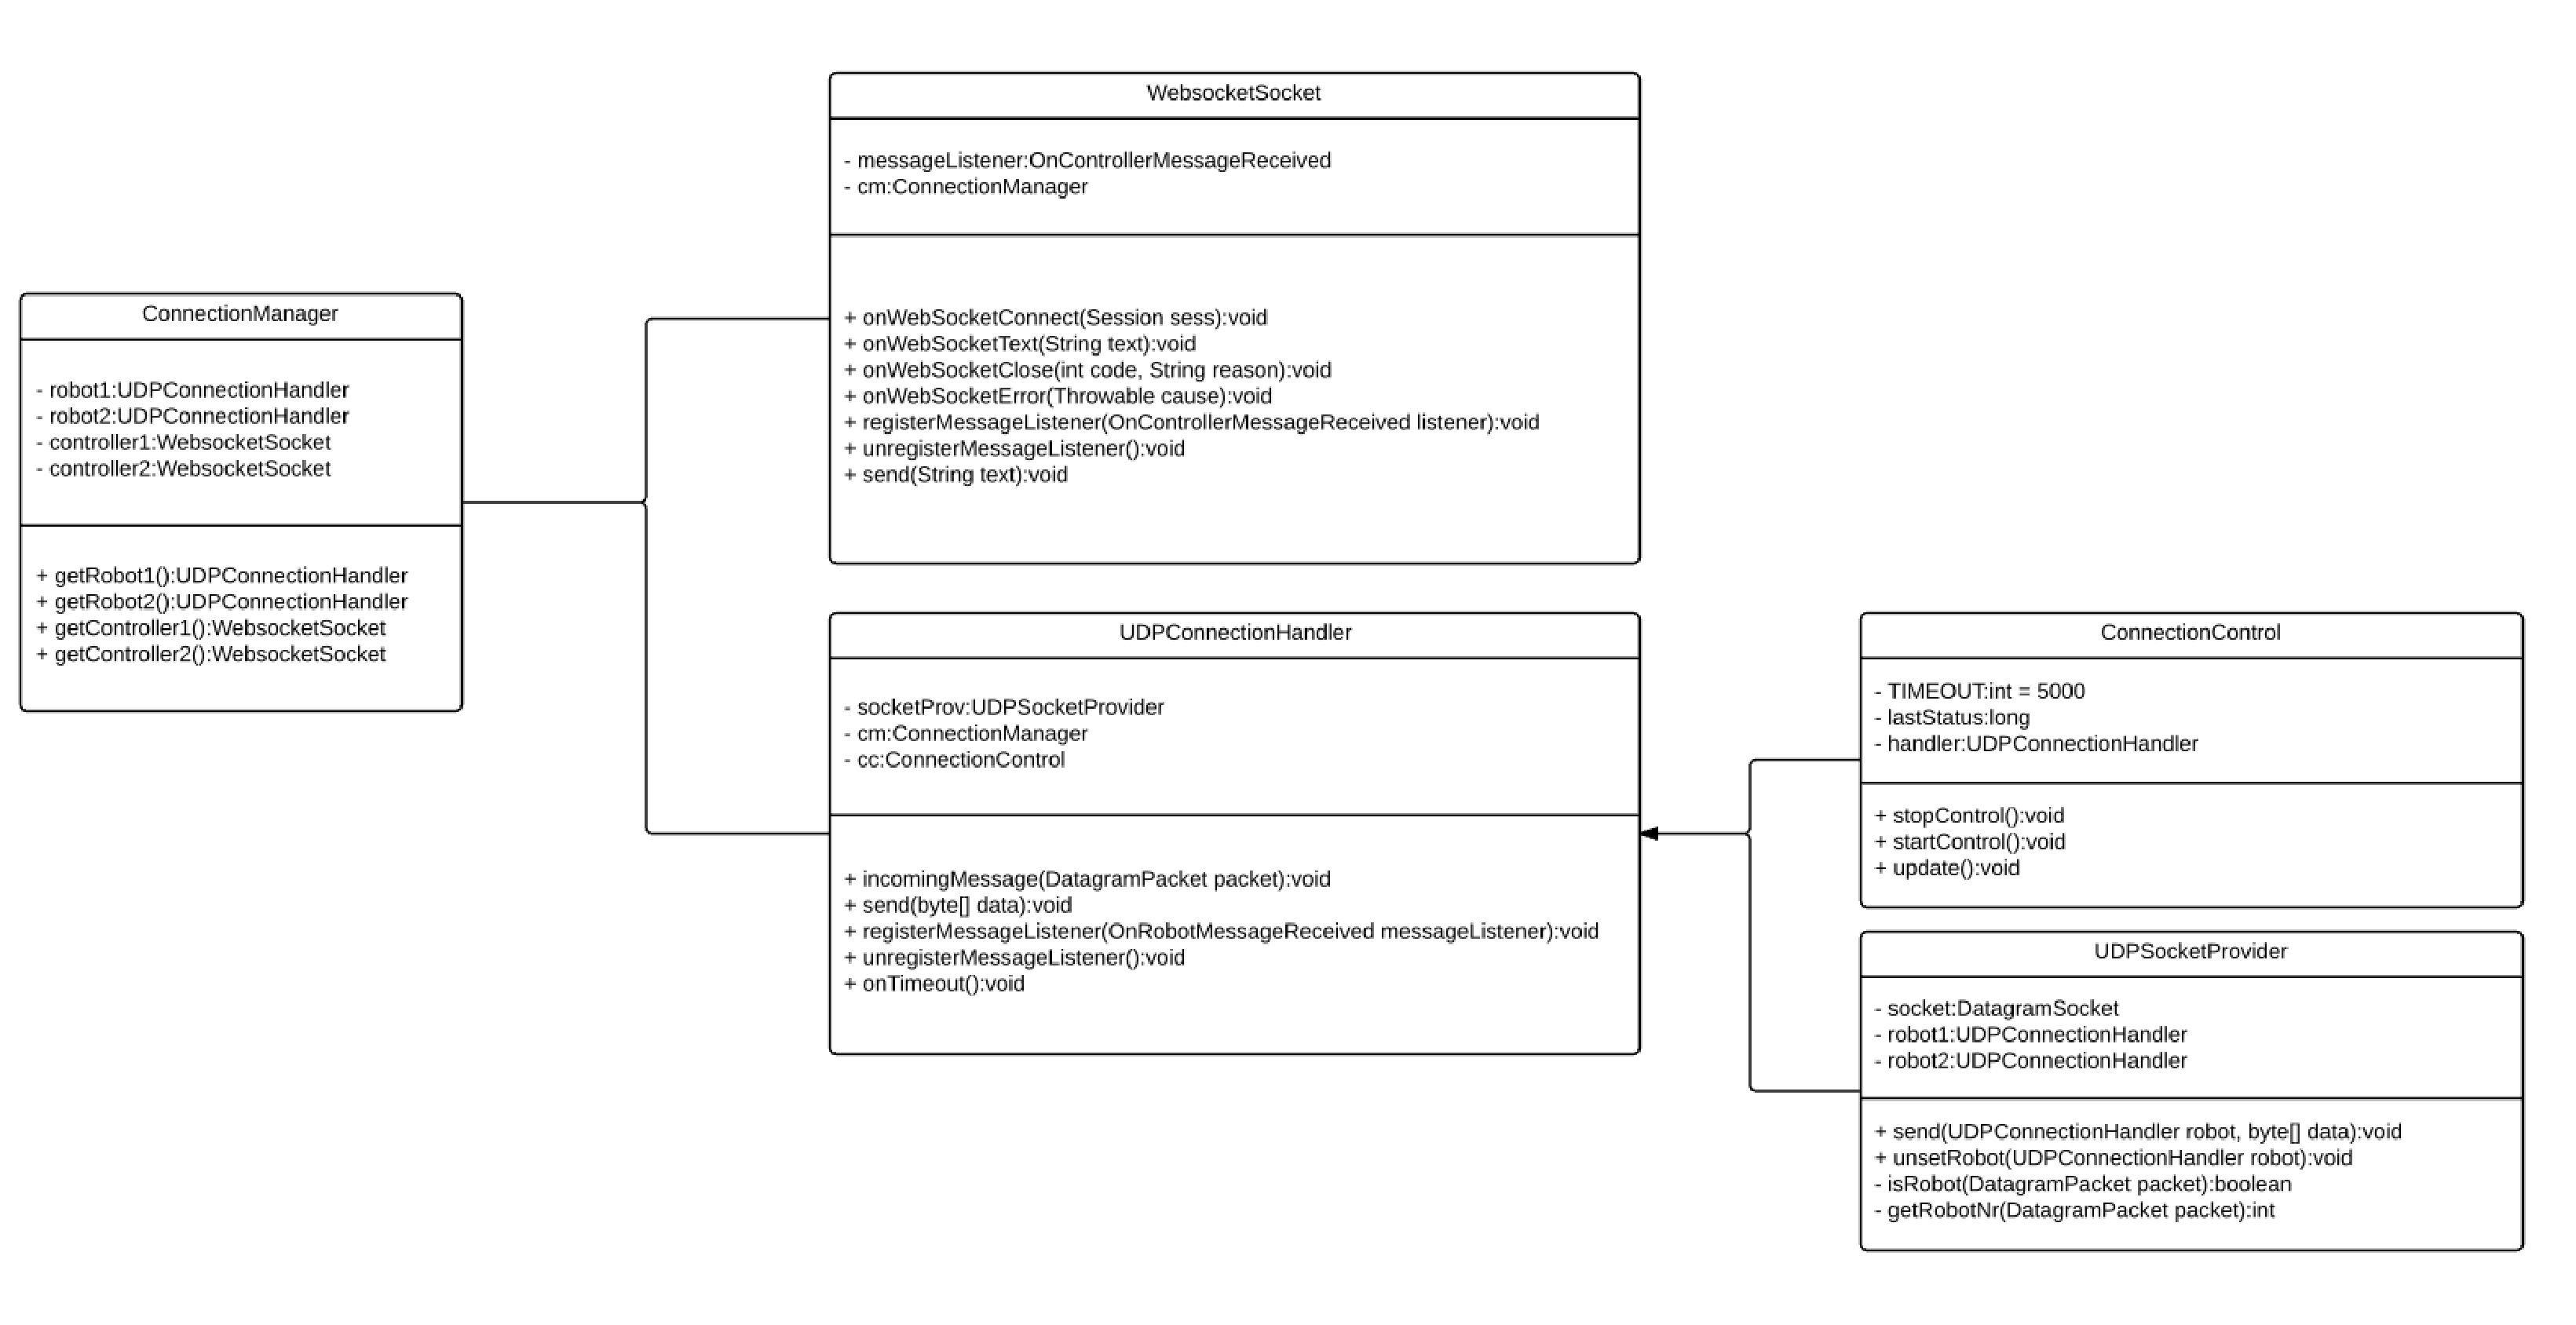
\includegraphics[width=\textwidth]{images/uml_verbindung.pdf}
	\caption{Klassendiagramm der Verbindungslogik}
	\label{fig:uml_verbindung}
\end{figure}



\subsection{Steueralgorithmen}
Da die verschiedenen Steuervarianten unterschiedliche Steuerparameter erzeugen ist es für jede einzelne davon notwendig, diese zu interpretieren und in eine Form zu bringen, die mit der Schnittstelle zum Roboter kompatibel ist. Auf diese wird in den nächsten Abschnitten genauer eingegangen. Das heißt, am Ende der Übersetzung müssen die Geschwindigkeiten der Motoren links und rechts und ob ein Schuss ausgelöst werden soll. Unabhängig der Steuervariante muss der Ausgangsbefehl anhand des vorherigen Befehls nachkorrigiert werden. Da die Motoren des Roboters eine im Vergleich zur Haftreibung der Räder hohe Beschleunigung aufweisen, müssen die Beschleunigungen begrenzt werden, um durchdrehende Räder und damit ein unkontrollierbares Verhalten der Steuerung zu vermeiden. 
Dies wird realisiert, indem ein maximal möglicher folgender Motorwert anhand des vorhergehenden Motorwertes errechnet wird. Die Berechnungsformel ist relativ simpel, der neue Wert darf um maximal einen festen Wert x größer sein als der alte Wert. Das ist dadurch zu begründen, dass für die Überschreitung der Haftreibung der Räder lediglich die dort wirkende Kraft ausschlaggebend ist, die wiederum aus der Beschleunigung der Räder resultiert. Dieser Wert x wurde nach einigen Testversuchen auf 10 festgelegt. Für den Fall, das beide gewünschten Motorenwerte über dem errechneten erlaubten Maximum liegen, muss anschließend das Verhältnis von linkem zu rechtem Motor angepasst werden, da sonst beide werte gleichgestellt werden, auch wenn diese sich zuvor unterschieden hätten. 
Zur Veranschaulichung dieser Korrektur folgt nun ein Beispiel:

Letzte Motorbefehle: \\
	links: 50 \\
	rechts: 50 
	
Neue Motorbefehle: \\
	links: 80 \\
	rechts: 70 
	
Neue Motorbefehle nach Korrektur (ohne Verhältnis nachzukorrigieren) \\
	links: 60 \\
	rechts: 60 
	
Wie man sieht wünscht der Benutzer durch seine Eingabe einen leichten Bogen nach rechts zu fahren, jedoch würden nach der Maximalwertkorrektur beide Motoren gleich schnell bewegt werden.

Nach Anpassung des Verhältnisses -- $\frac{links}{rechts} = \frac{8}{7}$ \\
	links: 60 \\
	rechts: $\frac{links}{\frac{8}{7}} = 52$


\subsubsection{Differential Steuerung}
Da die eingehenden Steuerparameter direkt die Motorenbefehle für Links und Rechts beinhalten (vgl. Abschnitt \ref{sec:differentialsteuerung}), ist hier keine weitere Interpretation notwendig. 

\subsubsection{RC-Remote Steuerung}
Die eingehenden Steuerparameter sind der Vorschub und die Richtung. Der Vorschub lässt sich direkt auf die Motoren übertragen, lediglich die Richtung muss mittels einer Formel berechnet werden. Der Interval indem sich der Wert der Richtung befindet ist [-50, 50]. An dieser Stelle bietet sich eine Exponentialformel an. 
Im Allgemeinen lautet diese: 
{\Large \[ratio_{LR} = a^{\frac{x}{50}}\]},
wobei der Parameter a bestimmt, wie groß das Verhältnis bei maximaler Auslenkung ist und x den momentanen Richtungswert angibt.
Nach einigen Testläufen wurde der Parameter a zu 2 bestimmt. Dadurch bewegt sich der linke Motor mindestens halb so schnell und maximal doppelt so schnell wie der rechte Motor.

\subsubsection{Webanwendung}
Diese Steuervariante hat einen bedeutenden Nachteil. Da die Eingangsparameter die momentan gedrückten Tasten sind (siehe Abschnitt \ref{sec:webanwendung}), gibt es keine Zwischenwerte für die Beschleunigung oder Richtung. Die Taste nach vorne bedeutet hierbei einen Motorschub für beide Seiten von 100\%. Für jede zusätzliche Richtungstaste, also links oder rechts, werden auf der dementsprechenden Seite 25\% abgezogen. Wird nur eine Richtungstaste ohne eine Beschleunigungstaste gedrückt, werden die Motoren auf -15\%/15\% bzw. 15\%/-15\% gesetzt, was einer Drehung auf der Stelle entspricht. Diese "Alles oder Nichts" Steuerung führt im Spiel zu einer nicht flüssigen, jedoch durch die Möglichkeit der Drehung auf der Stelle zu einer annehmbaren Steuerung.

\subsection{Bildübertragung}
Wie in der Schnittstellenbeschreibung in Kapitel \ref{sec:schnittstelle} beschrieben, werden die Bilddaten vom Roboter an die Statusnachrichten angehängt. Hierbei kennzeichnen die Bytes FF D8 den Beginn eines neuen Frames. Diese Kombination tritt in JPEG-kodierten Bildern immer nur am Anfang des Bildes auf, wodurch es möglich ist, Bilddaten über mehrere Pakete zu verteilen. Diese Daten werden dann in der Player-Klasse gepuffert, bis das Bild vollständig ist. Anschließend wird es noch base64 kodiert und sofort an die Controller weiter gesendet und nicht mit den regelmäßigen Statusbefehlen, um keine unnötige Zeitverzögerung einzubauen. Die base64 Kodierung wurde im Gegensatz zur einfachen Byte-Orientierten übertragen bevorzugt, damit an mit den Controllern in einer höheren Datenabstraktionsebene kommuniziert werden kann. Das vereinfacht den Code vor allem in der Webanwendung, da diese in Javascript implementiert ist. Ein großer Nachteil dieser Kodierung ist der größere Speicherbedarf, der die Übertragung aufgrund höheren Traffics langsamer macht und dadurch zu Verzögerungen führt, die letztendlich im Verlust der Steuerbarkeit resultieren können. Nach ersten Tests ist die Bildrate vom Roboter jedoch so gering, dass diese wenigen Frames rechtzeitig übertragen werden können. Zusätzlich sind die Frames in einer Größenordnung, in der 33 \% Mehrbedarf noch zu keiner Netzwerküberlastung führen.



\subsection{Torfindung}
Mit der Torfindung ist der Vorgang gemeint, um die Ladestation, die im Tor integriert ist zu finden und selbstständig anzufahren. Über die Statusmeldungen des Roboters erfährt der Server wie hoch der Akkustand des Roboters ist. Sobald der Roboter ein Minimum des Akkustands unterschreitet, greift die Torfindung ein. Diese wird in der Klasse EnergyManager implementiert (siehe Abb. \ref{fig:uml_energymanager}). Dabei wird die Torfindung sofort aktiviert, wenn sich ein Roboter mit dem Server verbindet und nicht erst wenn noch ein Controller hinzu kommt. Tritt der Fall ein, dass der Akku die Minimalschwelle unterschreitet, wird die Infrarot-Led über die Klasse BlinkTask angeschaltet. Über das "seeGoal" Flag (vgl. Schnittstellenbeschreibung, Kapitel \ref{sec:schnittstelle}) kann erkannt werden, ob das zum Roboter gehörende Tor in Sicht ist. Bekommt der Server vom Roboter drei aufeinander folgende Stati, in denen der Roboter meldet, dass das Tor in Sicht ist, dann fährt der Roboter rückwärts (Rückwärts, weil die Ladekontakte an der Rückseite des Roboters angebracht sind). Ist der Roboter vom eigenen Tor abgewandt, beginnt sich der Roboter zu drehen, solange bis entweder mindestens ein Status mit positiver Rückmeldung kommt, oder bis ein Timeout abgelaufen ist. Um die Drehung zu unterbrechen genügt deswegen bereits ein Status mit einer Sichtung, um die Möglichkeit einer korrekten Sichtung nicht durch zu schnelles drehen sofort zu verwerfen. Der Timeout bewirkt, dass sich der Roboter nicht endlos um sich selbst dreht, falls er außerhalb des Abstrahlwinkels der LED ist. Tritt ein Timeout auf, fährt der Roboter wenige Sekunden in die aktuelle Richtung, um seine Ausgangsposition zufällig zu ändern. Nach diesem Prinzip wird früher oder später die LED erkannt und das Tor und damit die Ladestation kann angefahren werden. 
Der Nachteil bei dieser Implementierung ist natürlich die unsichere Verhaltensweise des Roboters, wenn er außerhalb der LED-Reichweite ist. Diese führt im Worst-Case zu einer kompletten Entladung bis zur Bewegungsunfähigkeit, bevor die Station gefunden wurde. Da der Großteil des Spielfelds jedoch von den LEDs abgedeckt wird, ist dieser Fall unwahrscheinlich. Ein Vorteil dieser Methode im Gegensatz zu zum Beispiel einer Kamera basierten Positionsbestimmung ist die unabhängigkeit des Spielfelds. Lediglich die LED muss am Tor vorhanden sein, jedoch keine speziellen Konturen oder andere feste Muster, an denen der Roboter sich mithilfe der Kamera orientieren kann. Abgesehen davon ist die Torfindung mittels IR-LED vergleichsweise einfach zu realisieren.

\begin{figure}[h]
	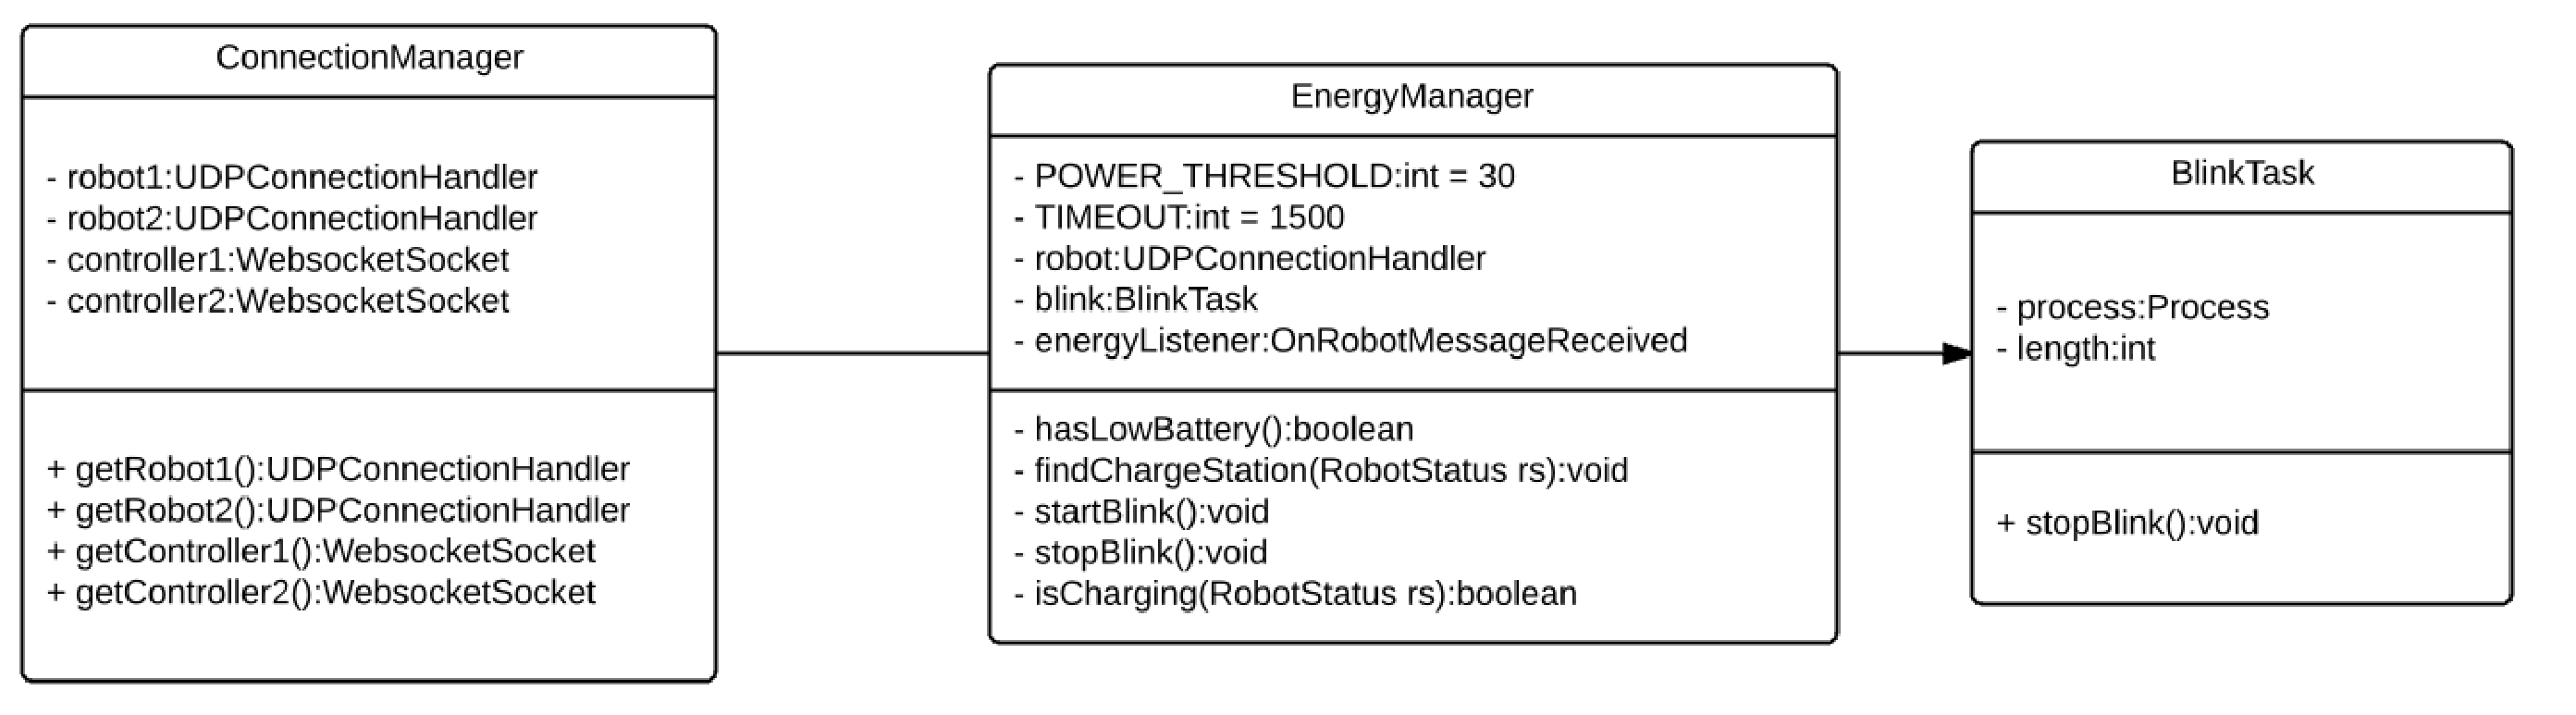
\includegraphics[width=\textwidth]{images/uml_energymanager.pdf}
	\caption{Klassendiagramm der Torfindung}
	\label{fig:uml_energymanager}
\end{figure}


\section{Ladestation}



\subsection{Infrarot-LED}
\label{sec:infrarot_led}
\subsection{Torerkennung}

\section{Webanwendung}
\label{sec:webanwendung}

\section{Android-Anwendung}
\subsection{RC-Remote Steuerung}
\subsection{Differential Steuerung}
\label{sec:differentialsteuerung}


% ...

\chapter{Fazit und Ausblick}
\label{ch:fazit}

Zum Ende der Arbeit erfolgt nun ein Fazit, indem auf die in der Einleitung definierten Ziele noch einmal eingegangen und diskutiert werden soll, ob die Vorgehensweise zieldienlich war. Anschließend gibt es einen Ausblick auf mögliche Erweiterungen und Verbesserungen der bestehenden Komponenten.

\section{Fazit}
Das Ziel der Arbeit war es, eine Steuerung für einen eigens entwickelten Roboter zu entwerfen, die es dem Benutzer ermöglicht mit seinem Smartphone oder Laptop den Roboter vor Ort, oder mithilfe der Kameraübertragung zu steuern, damit ein Fussballspiel ermöglicht werden kann. Dabei spielt es eine tragende Rolle, dass die Rechtzeitigkeit im Sinne der Übertragungszeit für Kamerabild und Befehlslatenz sicher gestellt ist. Hierfür war es notwendig eine geeignete Übertragungstechnologie zu finden und die Schnittstelle zum Roboter effizient zu gestalten. Auch die Aufgabe, den Roboter wartungsfrei zu halten was den Ladevorgang angeht, galt es zu bewältigen. \\
Die verzögerungsfreie Bedienbarkeit des Roboters über die Steuercontroller bestätigt die Rechtzeitigkeit in Bezug auf die Steuerung. Dies war zu erwarten, da die maximale Verzögerung von 100ms (vgl. \ref{sec:wahl_frequenz}) zwischen dem Wunsch und dem Eintritt einer Richtungsänderung zu keiner merklichen Beeinträchtigung des Spielflusses führen. Die Kameraübertragung jedoch hat aufgrund der niedrigen Framerate des Roboters gewisse Verzögerungen. Diese Verzögerungen führen bei einer hohen Geschwindigkeit des Roboters zu erschwertem Handling, die jedoch nicht von der Übertragung, sondern von der Roboterhardware zu verantworten sind. \\
Die Aufgabe den Roboter selbstständig an die Ladestation zu führen wurde meiner Meinung nach nur teilweise erfüllt. So ist es zwar möglich die Ladestation zu finden und auch anzufahren, jedoch hängt der Erfolg noch am Treffen der Ladekontakte. Da dies jedoch nur äußere Umstände sind, die von einer geschickteren Ladestation ausgemerzt werden könnten und die Station ja tatsächlich gefunden wird, halte ich diesen Punkt für wenig relevant, da er sich außerhalb des Interessengebiets befindet. \\
Somit lässt sich abschließend sagen, dass es durchaus möglich ist einen eigens entwickelten Fussballroboter ohne für den Nutzer erkennbare Verzögerungen zu steuern. Lediglich die Bildübertragung bringt eine gewisse Unrechtzeitigkeit ins Spiel, die aber vermutlich nicht an der Übertragung von Server zu Controller hängt, sondern an der Übertragungskapazität des Roboters. Wäre diese höher ausgefallen, hätte man sich sicherlich für ein Streamingprotokoll entscheiden müssen.\\
Die Anforderungen für diese Arbeit wurden jedoch zufriedenstellend erfüllt. Es wurde eine Steuerung für ein Roboter Fussballspiel entwickelt, bei dem die Roboter mithilfe von mobilen Endgeräten gesteuert werden.





\section{Ausblick}

Das Thema Steuerung von Robotern bietet generell viel Spielraum wenn es um Erweiterungen geht. Zunächst wird jedoch auf die bereits verwendeten Komponenten eingegangen.\\
Auf die Ladestation in Bezug auf das Design der Kontakte wird im Nachfolgenden nicht weiter eingegangen, da dies den Rahmen des eigentlichen Themas zu sehr übertreten würde. Jedoch wäre für die Torfindung an sich eine Positionsbestimmung des Roboters sehr hilfreich. Der Roboter müsste sich nicht ständig neu orientieren und könnte auf Anhieb den richtigen Weg zur Station finden. Dies ließe sich zum Beispiel mit einer über dem Spielfeld hängenden Kamera realisieren.  \\
Auch die Torerkennung bietet noch Verbesserungspotenzial. So könnte man die Tore mit Torkameras ausstatten, die den Ball erkennen. Das schließt Fehlerkennungen durch Rempler oder Fremdkörper aus. \\

Führt man diesen Gedanken Positionsbestimmung weiter, so wäre es dadurch auch möglich eine zentrale Steuerung seitens des Servers zu entwickeln. Hierbei würde der Server alle Steuerbefehle anhand der aktuellen Position des Roboters errechnen und diese an den Roboter senden, also eine Art Computergegner, um das Spiel auch ohne zweiten menschlichen Gegner spielen können. \\
Die Funktion den Roboter von außerhalb des Universitätsnetzwerks zu steuern ist zwar vorhanden, jedoch benötigt der Server hierfür auch eine öffentliche IP-Adresse. Wird ihm eine solche zugeteilt, wäre die Teilnahme am Spiel von jedem Ort mit Internetzugang möglich.
% ...

\chapter{Anhang}
\label{ch:anhang}

\begin{figure}[h]
	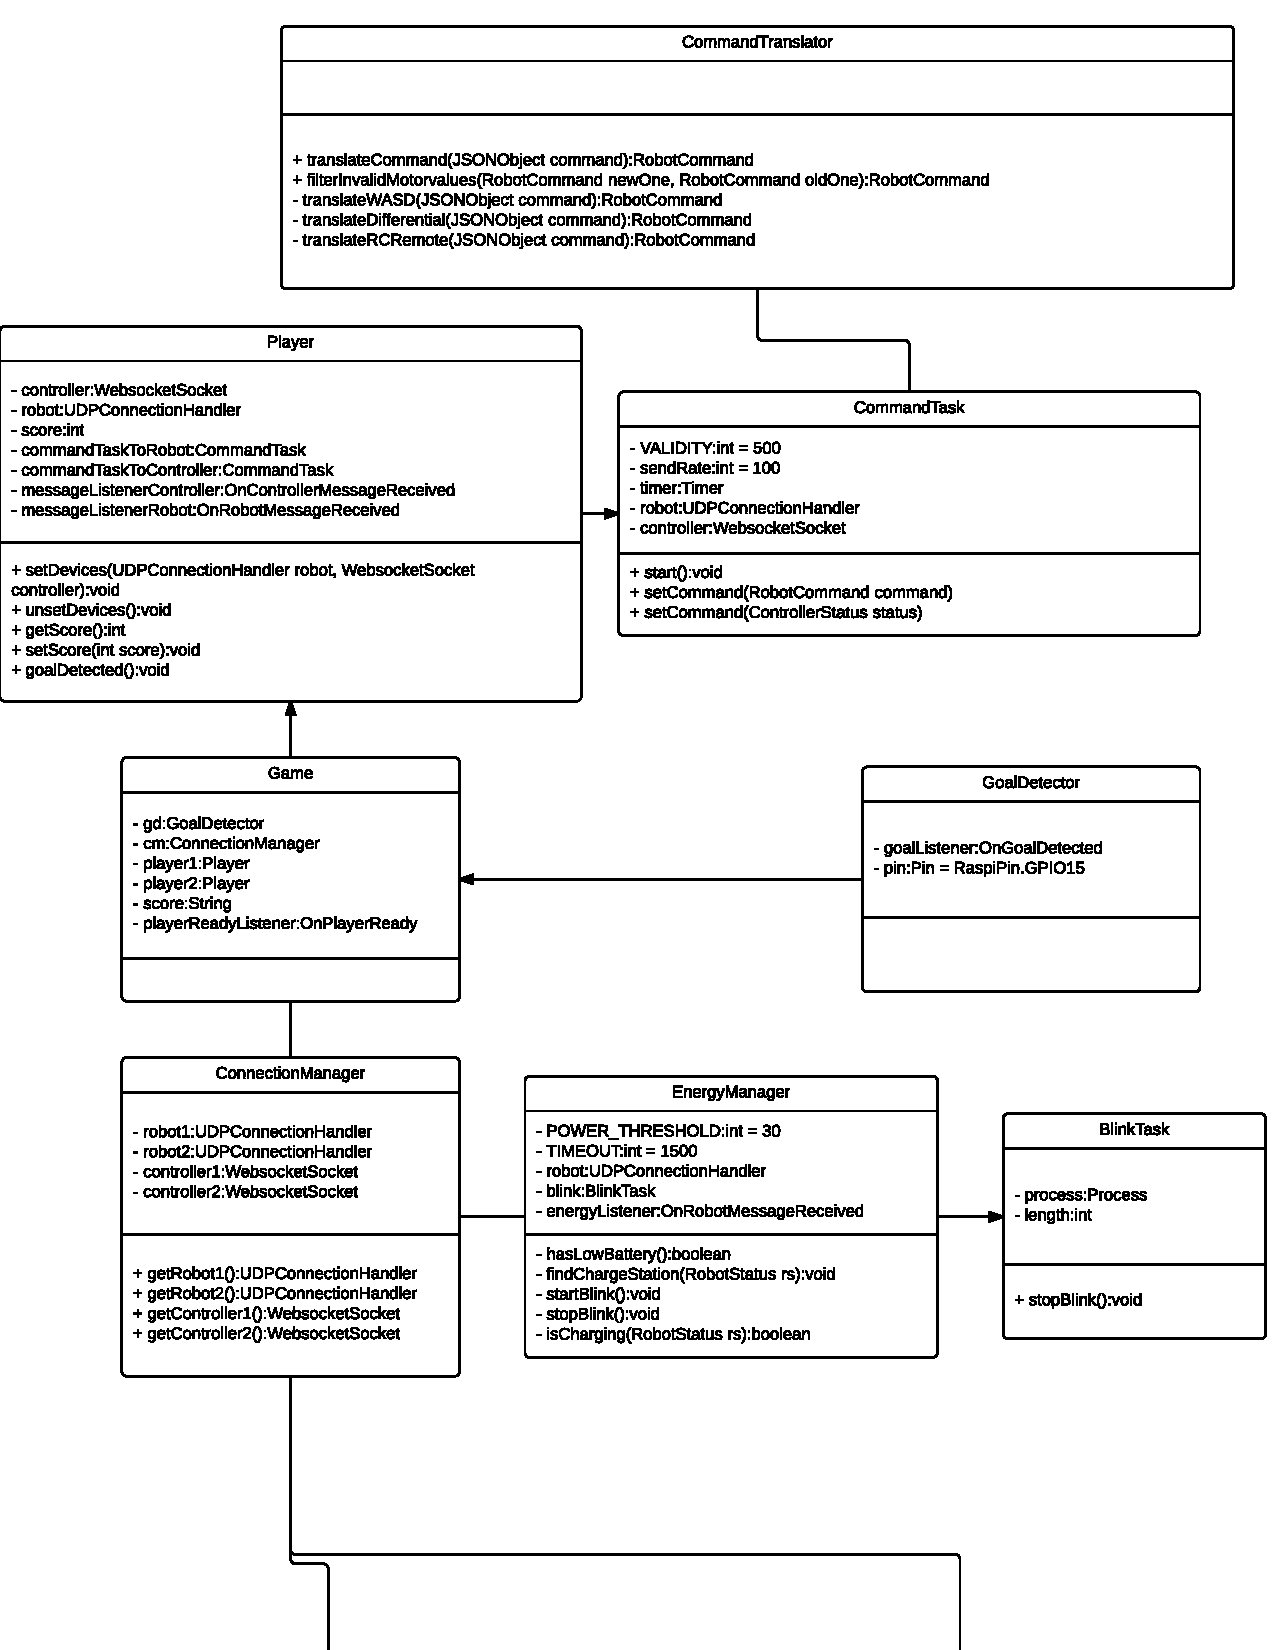
\includegraphics[page=1,width=.7\textwidth]{images/uml_software_all.pdf}

\end{figure}
\begin{figure}[h]
	\includegraphics[page=2,width=.7\textwidth]{images/uml_software_all.pdf}
	
	\caption{Klassendiagramm des Servers}
	\label{fig:server_uml_all}
\end{figure}
% ...

\chapter{Literaturverzeichnis}
\label{ch:literaturverzeichnis}
% ...


\backmatter %%%%%%%%%%%%%%%%%%%%%%%%%%%%%%%%%%%%%%%%%%%%%%%%%%%%%%%%%%%%%%%%%%%

\null\cleardoublepage

%\cite{*}
%\bibliographystyle{dinat} %first referenced
\bibliography{../literature/references.bib}

\cleardoublepage
\clearscrheadfoot
\ihead{Name: \theauthor}
\ohead{Matrikelnummer: \matrikelnr}
\cfoot{\pagemark}

\minisec{Erklärung}

Ich, \theauthor, Matrikelnummer \matrikelnr, erkläre, dass ich die Arbeit
selbständig verfasst und keine anderen als die angegebenen Quellen und
Hilfsmittel verwendet habe.

\vspace{2cm}

Ulm, den \dotfill

\hspace{10cm} {\footnotesize \theauthor}

\end{document}